
\subsection{Machine Learning Method}\label{section:ML}
We use the random forest algorithm to predict program outcome and fault type. A random forest is essentially an ensemble of single decision trees \cite{breiman2001random}. It captures different characteristics of the data, with each decision tree representing a model. One particular attractive aspect of random forest is that it allows us to analyze the importance of different features according to the information gain of each feature dimensions. We can use the information gain to rank the importance of each feature and therefore determine which features can be pruned.

%\begin{figure}[t]
%\begin{center}
%   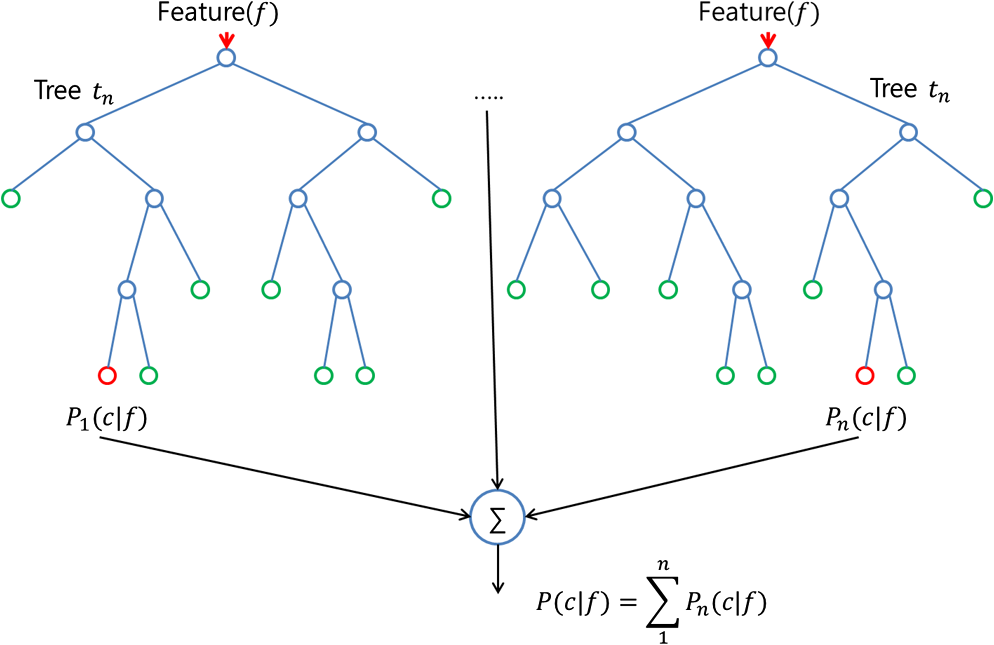
\includegraphics[width=0.95\linewidth]{./figures/rf.png}
%\end{center}
%   \caption{\footnotesize Random forests}
%\label{fig:rf}
%\end{figure}


%\begin{figure}[t]
%\begin{center}
%   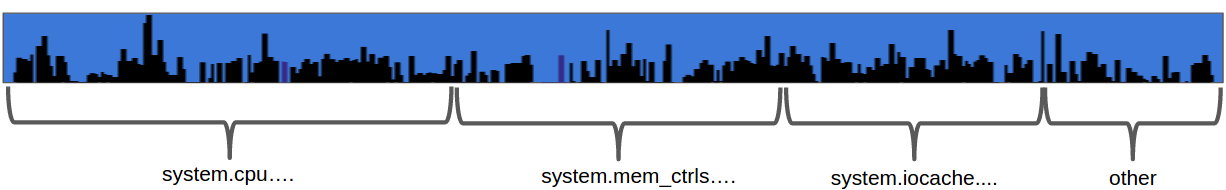
\includegraphics[width=0.95\linewidth]{./figures/feat_dist.png}
%\end{center}
%   \caption{\footnotesize Features in different components of the microachitecture.}
%   \vspace{-0.4cm}
%\label{fig:feat-dist}
%\end{figure}

%Figure~\ref{fig:feat-dist} shows features in different components of the microarchitecture.

We randomly select $60\%$ of instances for training and $40\%$ of instances for testing. Our dataset consists of $98,000$ data instances.